\PassOptionsToClass{hiresbb}{graphicx}
\documentclass[dvipdfmx,12pt,aspectratio=169]{beamer}

\usepackage{bxdpx-beamer}
\usepackage{pxjahyper}
\usepackage{minijs}
\usepackage{otf}
\renewcommand{\kanjifamilydefault}{\gtdefault}

\usetheme{Berkeley}

%サイドの配色設定
% ====== ここから追加 ======
% 全体の文字と背景
\setbeamercolor{normal text}{fg=black, bg=white}

% サイドバー(Berkeleyテーマで左側に出る部分)
\setbeamercolor{sidebar}{bg=gray!20, fg=black}

% サイドバー内のタイトルなど
\setbeamercolor{section in sidebar}{fg=black, bg=gray!30}
\setbeamercolor{subsection in sidebar}{fg=black, bg=gray!15}

% フレームタイトル(上の帯部分)
\setbeamercolor{frametitle}{bg=gray!40, fg=black}

% ブロック環境(block / exampleblock / alertblock)
\setbeamercolor{block title}{bg=gray!40, fg=black}
\setbeamercolor{block body}{bg=gray!10, fg=black}

% ====== ここまで追加 ======

\setbeamertemplate{navigation symbols}{}
\setbeamertemplate{footline}[frame number]


\usepackage[export]{adjustbox}
\usepackage{amsmath,amssymb,pifont}
\usepackage[main=english]{babel}
\usepackage{booktabs}
\usepackage{csquotes}
\usepackage[useregional]{datetime2}
\usepackage{graphicx}
\usepackage{siunitx}
\usepackage{ulem}
\usepackage{url}
\usepackage{xcolor}

\graphicspath{{./images/}} % search for images

% For better width adjustment with two columns
\newlength{\mytotalwidth}
\mytotalwidth=\dimexpr\linewidth-5mm
\newlength{\mycolumnwidth}
\mycolumnwidth=\dimexpr\mytotalwidth-5mm

% To-do lists
\newcommand{\notyet}{$\square$}
\newcommand{\done}{\rlap{\raisebox{0.3ex}{\hspace{0.4ex}\small \ding{52}}}{$\square$}}
\newcommand{\partly}{\rlap{\raisebox{0.3ex}{\hspace{0.4ex}\tiny \ding{52}}}{$\square$}}

\title{Progress}
\author{ShoMiyamoto}
\institute[NIAS]{Nagasaki Institute of Applied Science}
\date{\DTMdate{2025-10-17}}

\begin{document}
\begin{frame}\frametitle{}
\titlepage
\end{frame}

\section*{目次}
\begin{frame}\frametitle{発表の流れ}
\tableofcontents
\end{frame}

\section{trigger/I2C}
\subsection{ブロック環境の例}
\begin{frame}\frametitle{数式の例}

\[ \left( \int_0^\infty \frac{\sin x}{\sqrt{x}} dx \right)^2 = \frac{\pi}{2} \]
\end{frame}
\begin{frame}\frametitle{数式の例}
\begin{block}{2項係数に関する公式}
\[ (a + b)^{n} = \sum_{k = 0}^{n} \binom{n}{k} a^{k} b^{n-k} \]
\end{block}
\begin{exampleblock}{例}
公式に$a = 1, b = 1$を代入……
\[ 2^{n} = \sum_{k=0}^{n} \binom{n}{k} \]
\end{exampleblock}
\end{frame}

\subsection{アニメーションの例}
\begin{frame}\frametitle{PDFを使う利点}
\begin{itemize}
    \item<1-> Windows、macOS、Linux何でもOK
    \item<2-> すべてフリーのツールでできる
    \item<3-> \TeX $\to$ 複雑な数式もOK
\end{itemize}
\end{frame}

\section{ポイント}
\subsection{やることリスト}
\begin{frame}\frametitle{現在の状況}
\begin{block}{〇〇について}
\begin{itemize}
    \item[\done] やりきったこと
    \item[\partly] やりかけていること
    \item[\notyet] まだやっていないこと
\end{itemize}
\end{block}
\begin{block}{△△について}
\begin{itemize}
    \item[\done] やりきったこと
    \item[\partly] やりかけていること
    \item[\notyet] まだやっていないこと
\end{itemize}
\end{block}
\end{frame}

\subsection{図と箇条書きを並べる例}
\begin{frame}\frametitle{図を右に、箇条書きを左に}
\begin{columns}[totalwidth=\mytotalwidth]
\begin{column}[T]{0.3\mycolumnwidth}
\begin{itemize}
    \item こんな感じ
    \item 比率を変えるには、\texttt{0.3}と\texttt{0.7}を増減させる
\end{itemize}
\end{column}
\begin{column}[T]{0.7\mycolumnwidth}
\centering
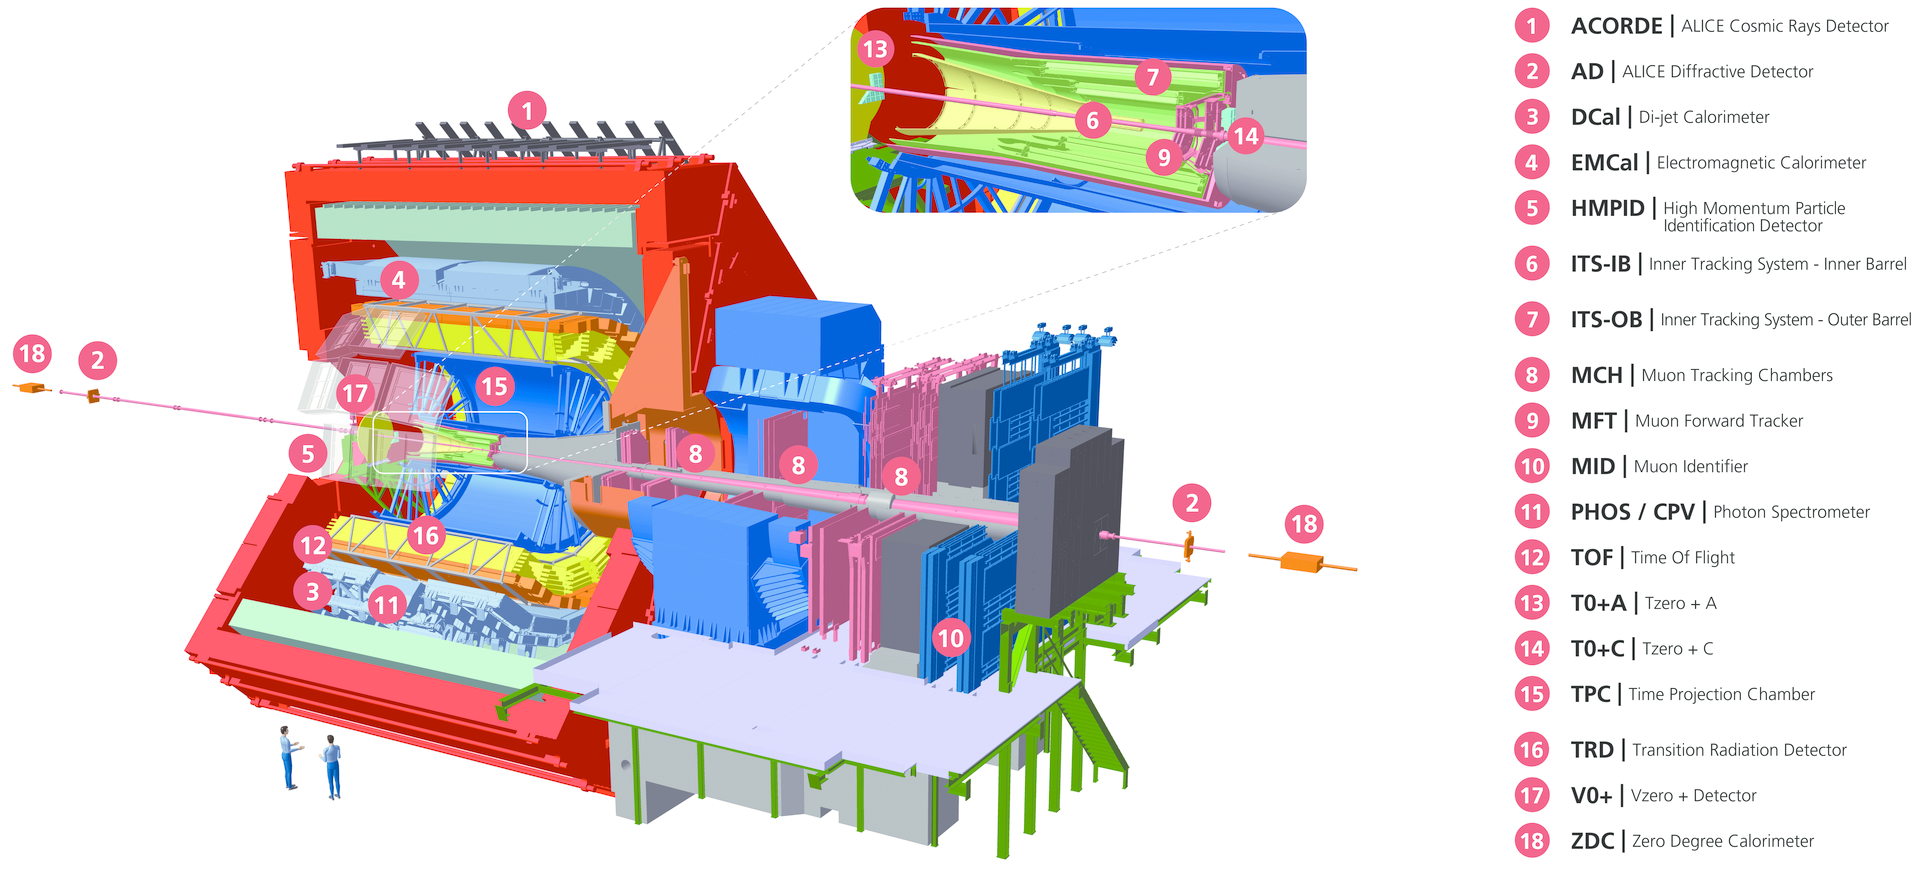
\includegraphics[width=0.7\mycolumnwidth]{ALICE-Run3.png}
\end{column}
\end{columns}
\end{frame}
\begin{frame}\frametitle{図を右に、箇条書きを左に}
\begin{columns}[totalwidth=\mytotalwidth]
\begin{column}[T]{0.3\mycolumnwidth}
\begin{itemize}
    \item \texttt{T}を\texttt{c}に変えると高さ方向のレイアウトが中央揃えになる
\end{itemize}
\end{column}
\begin{column}[T]{0.7\mycolumnwidth}
\centering
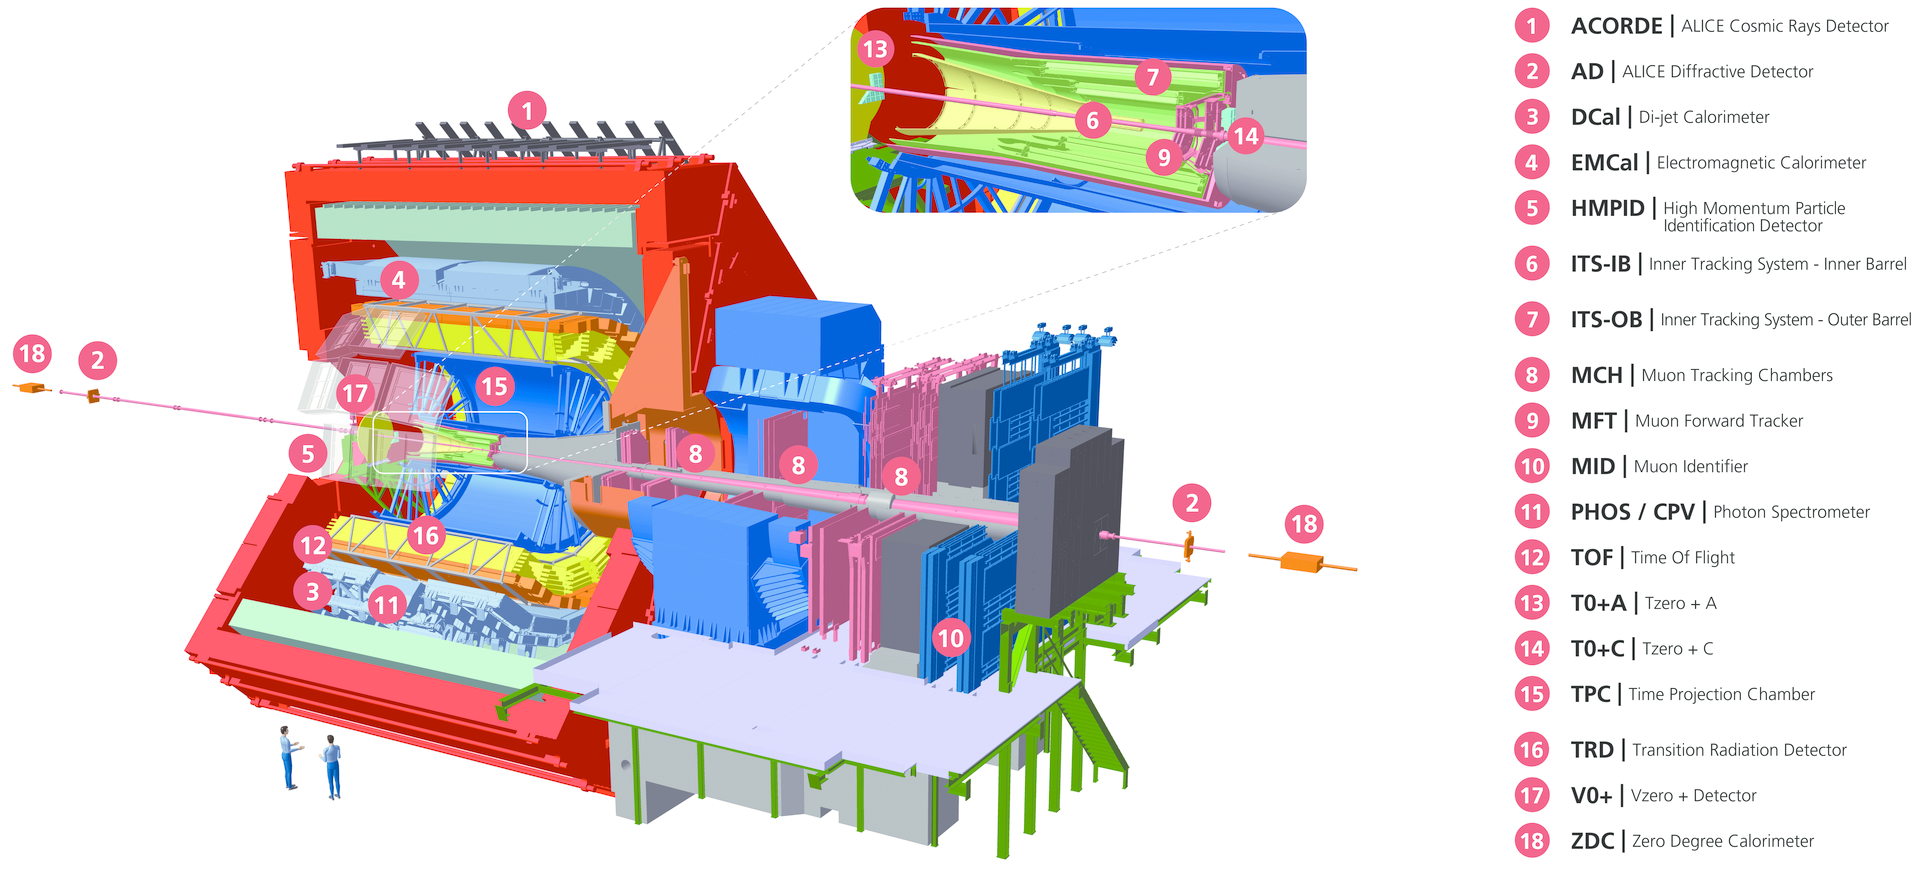
\includegraphics[width=0.7\mycolumnwidth]{ALICE-Run3.png}
\end{column}
\end{columns}
\end{frame}
\begin{frame}\frametitle{図を右に、箇条書きを左に}
\begin{columns}[totalwidth=\mytotalwidth]
\begin{column}[c]{0.3\mycolumnwidth}
\begin{itemize}
    \item \texttt{T}を\texttt{c}に変えた場合
\end{itemize}
\end{column}
\begin{column}[c]{0.7\mycolumnwidth}
\centering
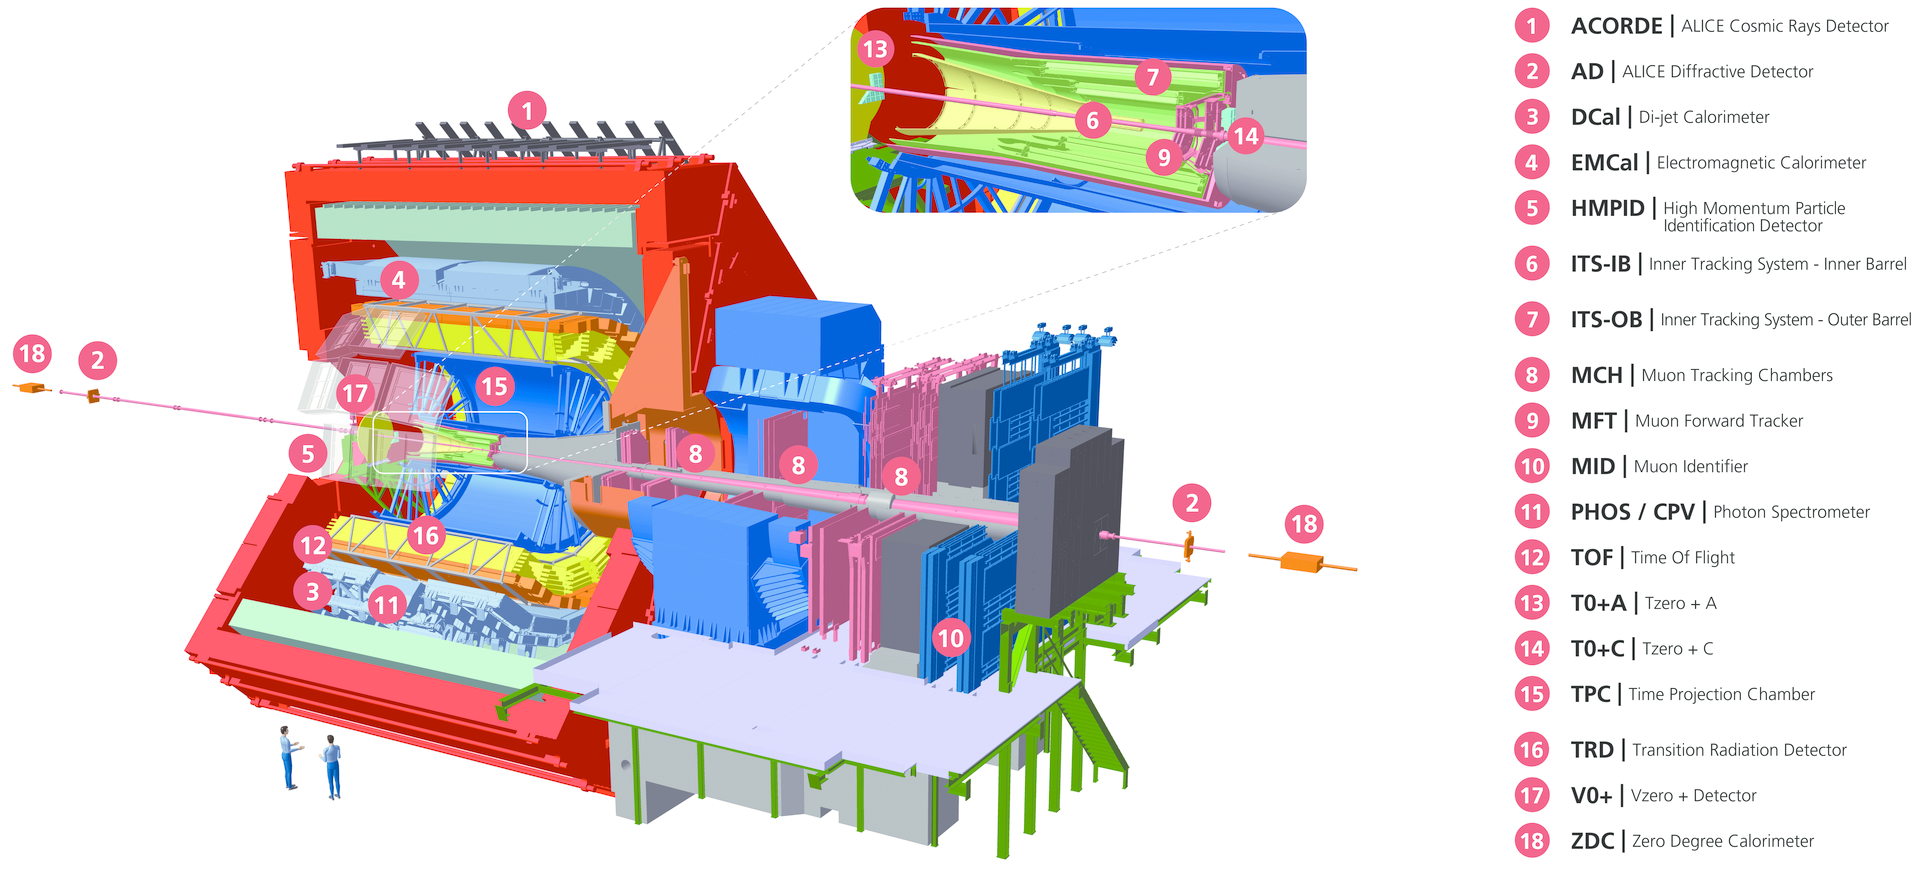
\includegraphics[width=0.7\mycolumnwidth]{ALICE-Run3.png}
\end{column}
\end{columns}
\end{frame}
\begin{frame}\frametitle{箇条書きを右に、図を左に}
\begin{columns}[totalwidth=\mytotalwidth]
\begin{column}[T]{0.6\mycolumnwidth}
\centering
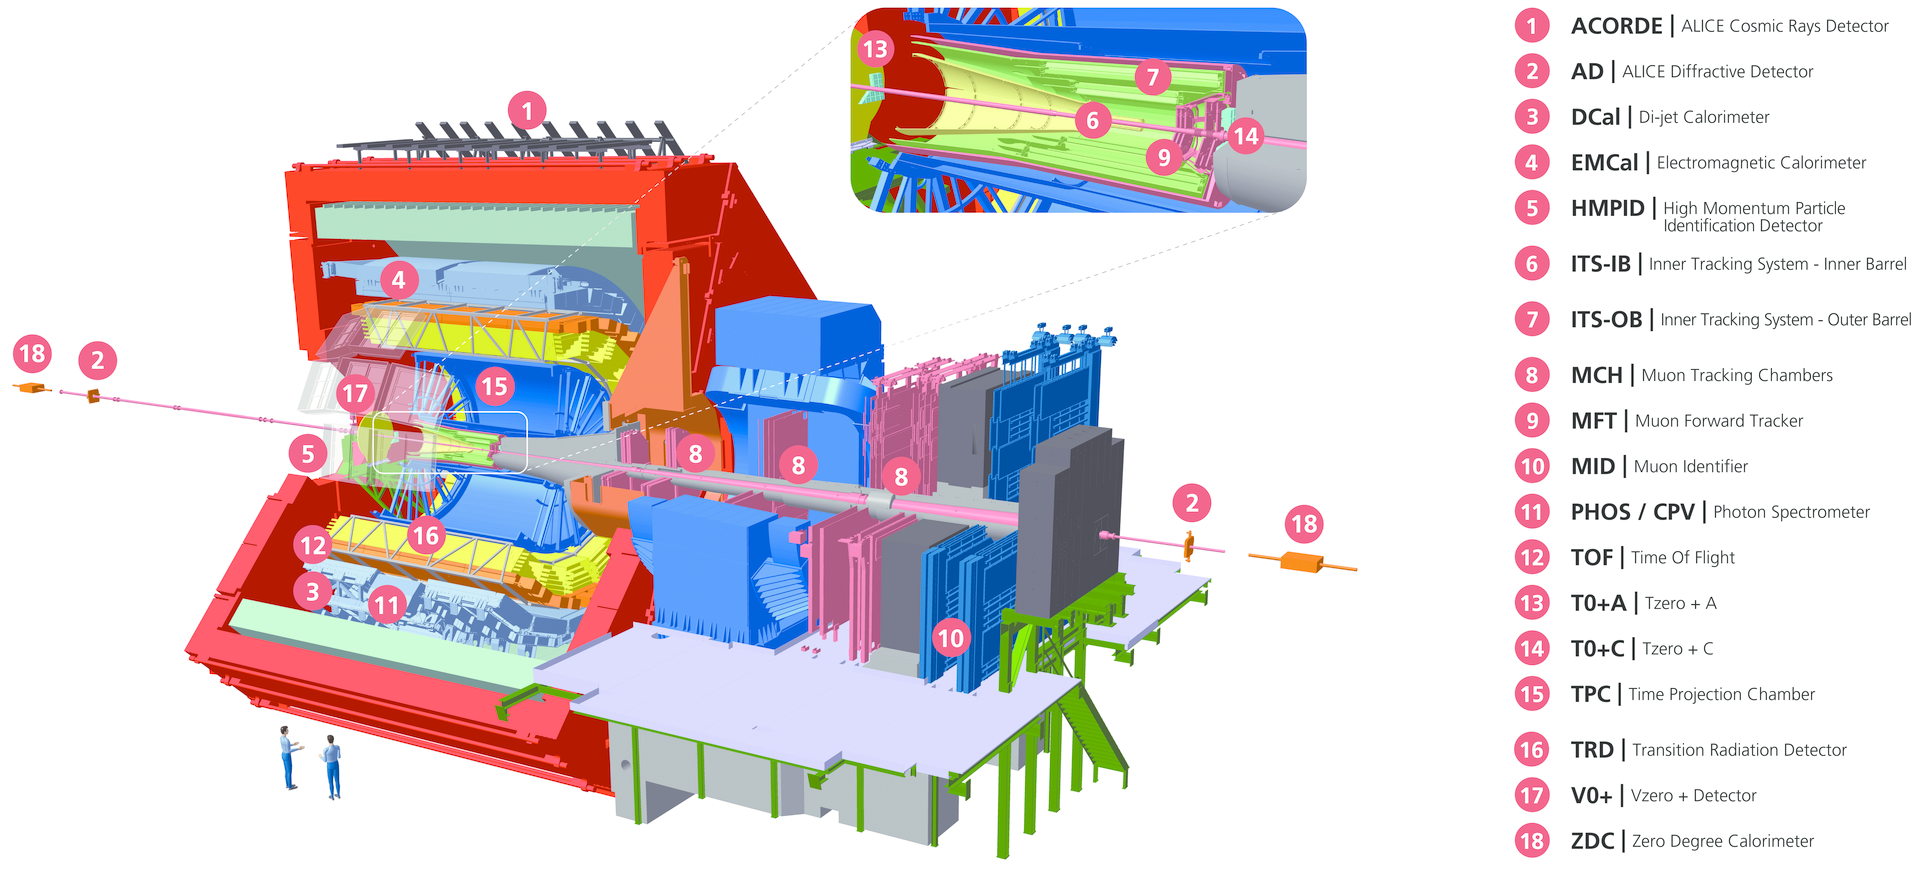
\includegraphics[width=0.6\mycolumnwidth]{ALICE-Run3.png}
\end{column}
\begin{column}[T]{0.4\mycolumnwidth}
\begin{itemize}
    \item 記述の順番を変えれば表示の順番も変わる
\end{itemize}
\end{column}
\end{columns}
\end{frame}
\subsection{その他のポイント}
\begin{frame}\frametitle{細かいコツ}
\begin{itemize}
    \item 単位付きの量を表記するときは\texttt{siunitx}を使おう(例:\SI{1}{nm})
    \item 大文字と小文字に気をつけよう(例:\SI{1}{mV}と\SI{1}{MV})
    \item 画像は\texttt{images/}ディレクトリにアップロードしよう \begin{itemize}
        \item トップレベルのディレクトリを散らかさない
        \item 参照するときは\texttt{images/ALICE-Run3.png}でも\texttt{ALICE-Run3.png}でもOK
    \end{itemize}
    \item 大きな画像の一部を切り抜いて載せたい場合は、画像編集アプリを使ってもいいけど、\texttt{adjustbox}も便利
\end{itemize}
\end{frame}
\end{document}
